\maketitle
\setcounter{page}{1}
\tableofcontents
\newpage
\pagenumbering{arabic}
\section{Theorie}
Atomkerne zerfallen, wenn das Verhältnis zwischen Anzahl von Neutronen und Protonen
bestimmte Grenzen überschreitet. Eine wichtige Größe zum Zerfall von Atomen in die
Halbwertszeit $T$. Diese bezeichnet den Zeitraum, in dem die Hälfte der instabilen Kerne
zerfallen ist. In diesem Versuch wird eine Methode diskutiert, die Halbwertszeit von Nukliden zu bestimmen,
deren $T$ in der Größenordnung Sekunden bis Stunden liegt. Da diese zu Beginn der Messung hergestellt
werden müssen, geschieht dies durch den Beschuss stabiler Kerne mit Neutronen, da diese die Coulomb-Barriere
nicht überwinden müssen. Im folgenden wird diese Kernreaktion betrachtet.

Sobald ein Neutron von einem Kern A aufgenommen wurde,  entsteht ein neuer Kern A*, den man Compound -
oder Zwischenkern nennt. Ihn unterscheidet von seinem Vorgänger die kinetische und Bindungsenergie
des Neutrons. Diese Energie verteilt sich auf viele Nukleonen, die dadurch in höhere Energiezustände
gebracht werden. Deswegen ist es nicht möglich, dass der Kern das neue Nukleon oder ein anderes abstößt.
Aus diesem Grund geht der Kern nach der Emmission eines $\gamma$ - Quants wieder in seinen Grundzustand über:
\begin{equation*}
    \ce{^{m}_{z}A} + \ce{^{1}_{0} n} \rightarrow \ce{^{m + 1}_{z}A^*} \rightarrow \ce{^{m + 1}_{z}A} + \gamma
\end{equation*}
mit m als Massenzahl und z als Kernladungszahl. Der neue Kern $\ce{^{m + 1}_{z}A}$ ist nicht mehr stabil,
da er mehr Neutronen als ein stabiler Kern enthält. Er zerfällt nach längerer Zeit nach folgender Gleichung:
\begin{equation*}
    \ce{^{m + 1}_{z}A} \rightarrow \ce{^{m+1}_{z+1}C} + \symup{\beta}^- + \symup{E_{kin}} + \overline{\symup{\nu}}_{\symup{e}}
\end{equation*}
mit $\overline{\symup{\nu}}_{\symup{e}}$ als Antineutrino. Der Massendefekt in der obigen Gleichung wird
durch die kinetische Energie von Elektron und Antineutrino ausgeglichen.

Der Wirkungsquerschnitt $\sigma$ gibt die Wahrscheinlichkeit an, mit der ein Neutron von einem stabilen Kern
absorbiert wird. Er ist definiert durch
\begin{equation}
  \sigma = \frac{u}{nKd}
  \label{eqn:1}
\end{equation}
mit $u$ als Anzahl der Treffer, $n$ als Anzahl Neutronen pro Sekunde und $d$ als Dicke und $K$ als Atome pro $\symup{cm}^3$
einer \SI{1}{\centi\meter\squared} breiten Folie. Der Wirkungsquerschnitt ist stark geschwindigkeitsanhängig.
Wenn die Geschwindigkeit des Neutrons hoch genug ist, dass die De-Broglie Wellenlänge klein gegen den Radius
des Kerns ist, kann geometrische Optik angewendet werden und es müssen keine Interferenzeffekte betrachtet werden.

Damit Resonanzabsorption auftritt

\section{Durchführung}
\subsection{Versuchsaufbau}
\subsection{Versuchsdurchführung}
\section{Auswertung}
\subsection{Zur mathematischen Behandlung der Messwerte}
Die gemessenen Vorgänge unterliegen einer Poission-Verteilung, der Fehler eines
Messwertes $x_i$ ist somit durch $\sqrt{x_i}$ gegeben. Die dargestellten Ausgleichsrechnungen
wurden durch die Funktion \textsc{curve-fit} aus dem \textsc{python}-Paket \textsc{scipy.optimise}
unter berücksichtigung des Fehlers durchgeführt.
\subsection{Nullmessung}
Es wurden innerhalb von \SI{900}{\second} \num{164} Ausschläge am Geiger-Müller-Zählrohr
gemessen. Dies entspricht einem Wert von $N_\symup{null} = \SI[per-mode=reciprocal]{0.18}{\per\second}$.
Dieser Wert ist zwar gering, aber gerade bei längeren Messintervallen statistisch
signifikant, sodass er von den Messwerten abgezogen werden muss.
\subsection{Messung von Indium}
\begin{figure}
  \centering
    \begin{subfigure}{0.7\textwidth}
    \centering
      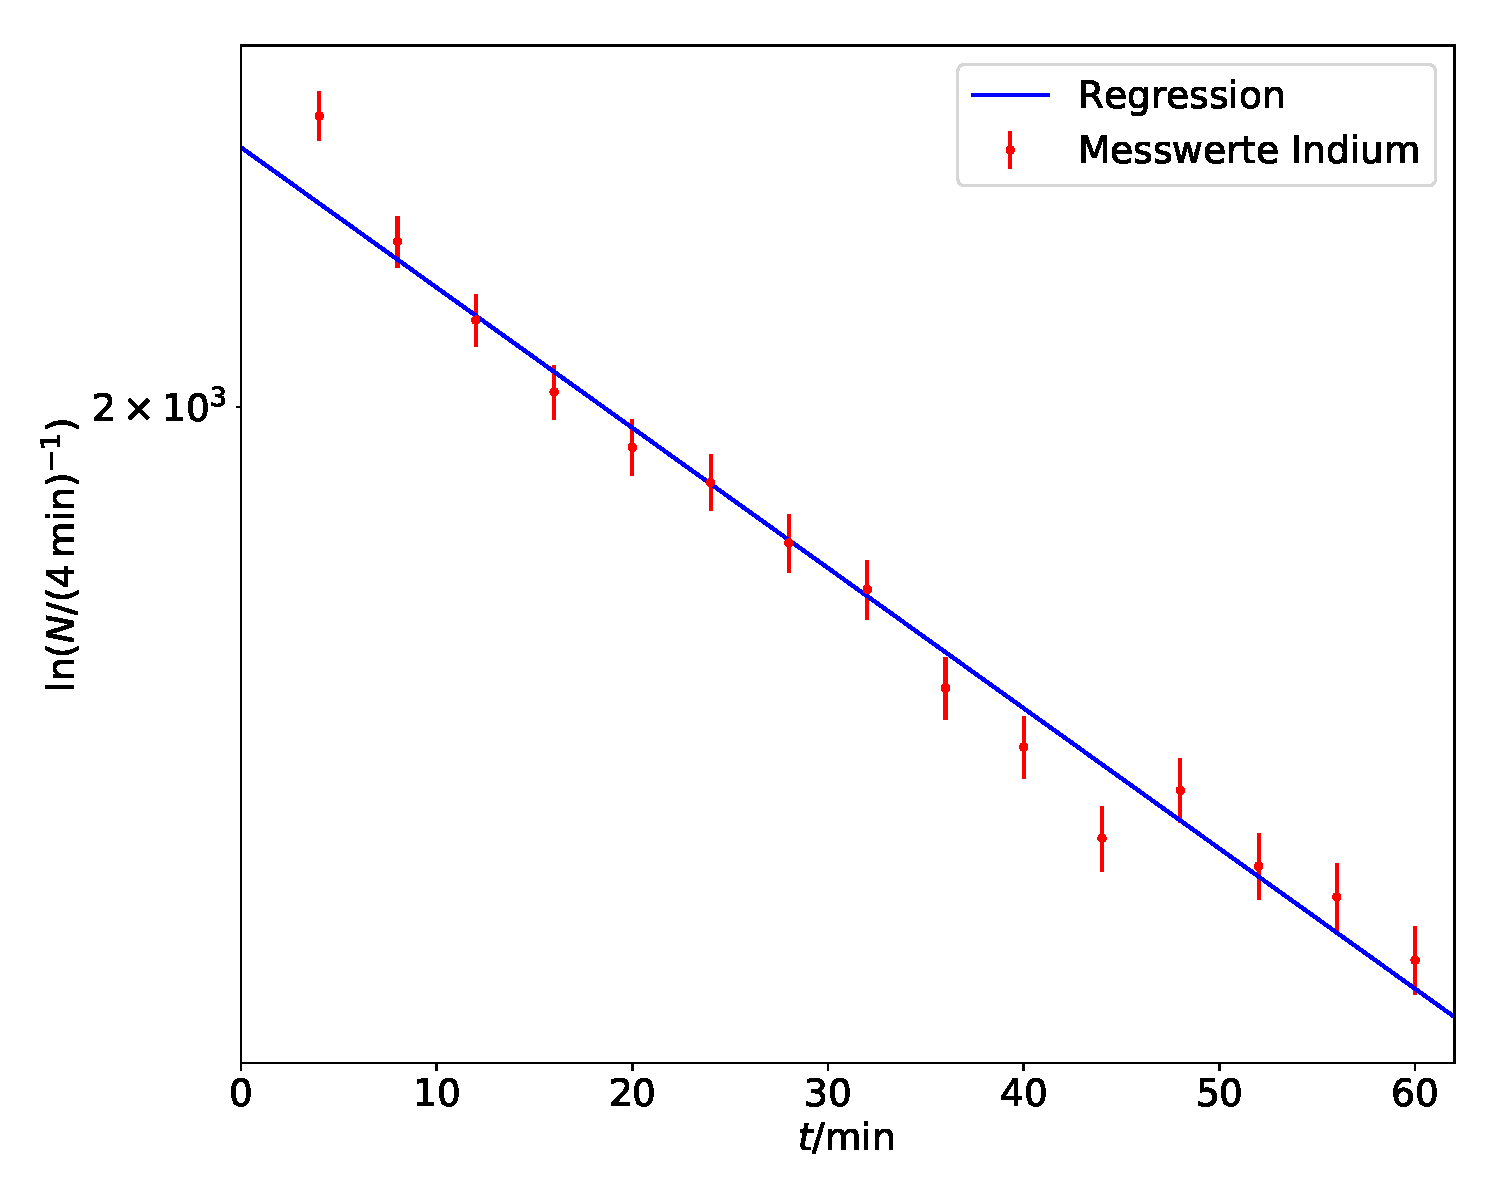
\includegraphics[width=\textwidth]{Indium.pdf}
      \caption{Grafische Darstellung der Messwerte mit Regression.}
      \label{fig:1}
    \end{subfigure}
    \begin{subtable}{0.25\textwidth}
      \centering
      \begin{tabular}{c c}
        \toprule
        t / \si{\minute} & N \\
        \midrule
        4 & 2584 \\
        8 & 2335 \\
        12 & 2192 \\
        16 & 2069 \\
        20 & 1979 \\
        24 & 1924 \\
        28 & 1833 \\
        32 & 1766 \\
        36 & 1632 \\
        40 & 1557 \\
        44 & 1448 \\
        48 & 1504 \\
        52 & 1416 \\
        56 & 1382 \\
        60 & 1314 \\
        \bottomrule
      \end{tabular}
      \caption{Messwerte.}
      \label{tab:1}
    \end{subtable}
    \caption{In Tabelle \subref{tab:1} sind die für das Isotop
    $\ce{^{116}In}$ gemessenen Werte eingetragen. Diese Werte sind
    nicht vom Nulleffekt bereinigt. In Grafik \subref{fig:1} findet sich die
    halblogarithmische Darstellung der vom Nulleffekt bereinigten Messwerte mit
    einer linearen Regression.}
  \end{figure}
  Die Messwerte finden sich in Tabelle \ref{tab:1}. Die Werte fallen mit einer
  Exponentialfunktion
  \begin{equation}
    N(t) = N_0 \symup{e}^{- \mu t}
    \label{eq:1}
  \end{equation}
  ab. Es bietet sich also eine lineare Regression mit einer Funktion
  \begin{equation*}
    n(t) = \ln{N_0} - \mu t
  \end{equation*}
  durch die logarithmierten Messwerte an. Aus \ref{eq:1} folgt weiterhin für die Halbwertszeit $T_{1/2}$:
  \begin{equation}
    T_{1/2} = \ln{\frac{1}{2}} \cdot -\mu^{-1}
  \end{equation}
  Es ergeben sich also folgende Konstanten:
  $N_0$:
  \begin{align*}
    \mu_\symup{In} =& \, \SI[per-mode=reciprocal]{1.91(8)e-4}{\per\second} \\
    N_{0\symup{, In}} =& \, \SI[per-mode=reciprocal]{10.3(2)}{\per\second} \\
    T_{1/2} =& \, \SI{60.3(25)}{\minute}.
  \end{align*}
Die Messwerte mit Fehler sowie die berechnete Regression finden sich in Abbildung \ref{fig:1}.
\subsection{Messung von Silber}
\begin{table}
  \centering
  \begin{tabular}{c c | c c | c c | c c}
    \toprule
    t / \si{\second} & N & t / \si{\second} & N & t / \si{\second} & N & t / \si{\second} & N \\
    \midrule
    8 & 146 & 120 & 21 & \sout{232} & \sout{6} & 344 & 6 \\
    16 & 120 & 128 & 18 & \sout{240} & \sout{11} & 352 & 3 \\
    24 & 86 & \sout{136} & \sout{22} & 248 & 10 & 360 & 4 \\
    \sout{32} & \sout{87} & 144 & 16 & \sout{256} & \sout{3} & \sout{368} & \sout{15} \\
    40 & 60 & \sout{152} & \sout{22} & \sout{264} & \sout{4} & 376 & 5 \\
    \sout{48} & \sout{58} & 160 & 17 & 272 & 10 & 384 & 5\\
    56 & 43 & 168 & 15 & 280 & 9 & \sout{392} & \sout{9}\\
    \sout{64} & \sout{51} & \sout{176} & \sout{5} & \sout{288} & \sout{5} & 400 & 2 \\
    72 & 34 & 184 & 11 & 296 & 9 & 408 & 5 \\
    80 & 24 & 192 & 12 & 304 & 10 & \sout{416} & \sout{9} \\
    88 & 24 & \sout{200} & \sout{13} & \sout{312} & \sout{6} & 424 & 5 \\
    \sout{96} & \sout{26} & 208 & 9 & 320 & 10 & & \\
    104 & 23 & 216 & 9 & 328 & 10 & & \\
    112 & 24 & \sout{224} & \sout{6} & 336 & 6 & & \\
    \bottomrule
  \end{tabular}
  \caption{Messwerte .}
  \label{tab:2}
\end{table}
Die Messwerte finden sich in Tabelle \ref{tab:2}. Messwerte, die deutlich als fehlerhaft
erkennbar sind, werden in den Berechnungen nicht beachtet und sind in der Tabelle
durchgestrichen. Die betrachteten Messwerte 

\section{Diskussion}

\newpage
\nocite{*}
\printbibliography
